\documentclass[12pt]{beamer}
\usepackage{amsmath,amssymb,caption,csquotes,float,tabularx}
\usepackage{minted}
\usepackage[utf8]{inputenc}
\usepackage[english]{babel}
\usepackage[backend=bibtex]{biblatex}
\addbibresource{spmr.bib}
\captionsetup[figure]{labelsep=period}
\captionsetup[table]{labelsep=period}
\definecolor{bg}{rgb}{0.95,0.95,0.95}
\hypersetup{
    colorlinks=true,
    linkcolor=blue,
    filecolor=blue,      
    urlcolor=blue,
    citecolor=cyan,
}
\usemintedstyle{emacs}
\usetheme{Madrid}
\begin{document}
\title{Qualcomm\textsuperscript{\textregistered} Cloud Al 100}
\subtitle{SoC Product Manual Review Presentation}
\author{Yihua Liu}
\institute{UM-SJTU Joint Institute}
\date{\today}
\begin{frame}
    \titlepage
\end{frame}
\section{Product Overview}
\begin{frame}{Product Overview}
    \begin{columns}
        \begin{column}{0.5\linewidth}
            \begin{figure}[H]
                \centering
                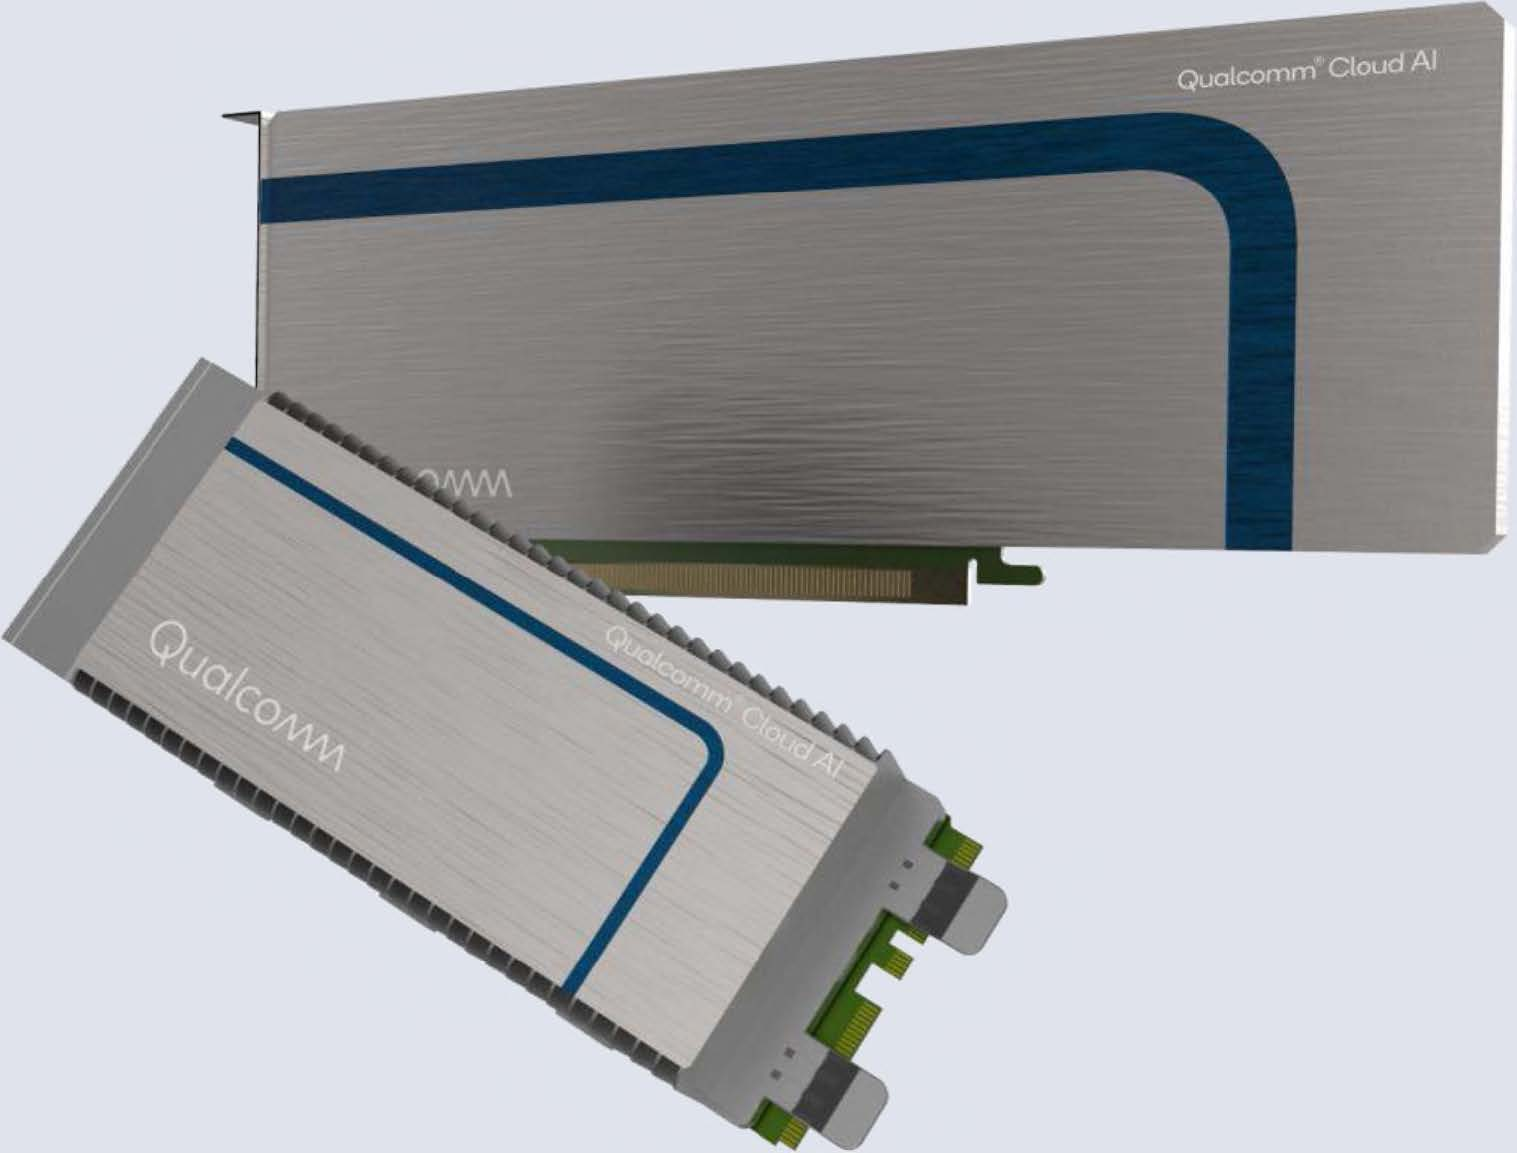
\includegraphics[width=0.8\columnwidth]{2.jpg}
            \end{figure}
            \begin{figure}[H]
                \centering
                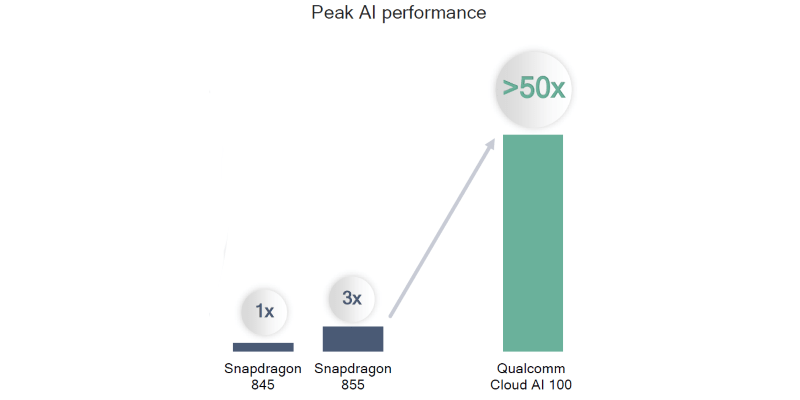
\includegraphics[width=0.8\columnwidth]{3.png}
                \caption{\scriptsize Peak AI performance \cite{eetimes2019}.}
            \end{figure}
        \end{column}
        \begin{column}{0.5\linewidth}
            \begin{itemize}
                \scriptsize
                \item Research starts since 2016
                \item Qualcomm's most advanced low-power and high performance AI processing
                \item Powerful and efficient processing speeds: More than 10x performance per watt over the industry's most advanced AI inference solutions deployed today
                \item Specifically designed for processing AI inference workloads
            \end{itemize}
        \end{column}
    \end{columns}
\end{frame}
\section{Application Overview}
\begin{frame}{Application Overview}
    \begin{columns}
        \begin{column}{0.5\linewidth}
            \begin{figure}[H]
                \centering
                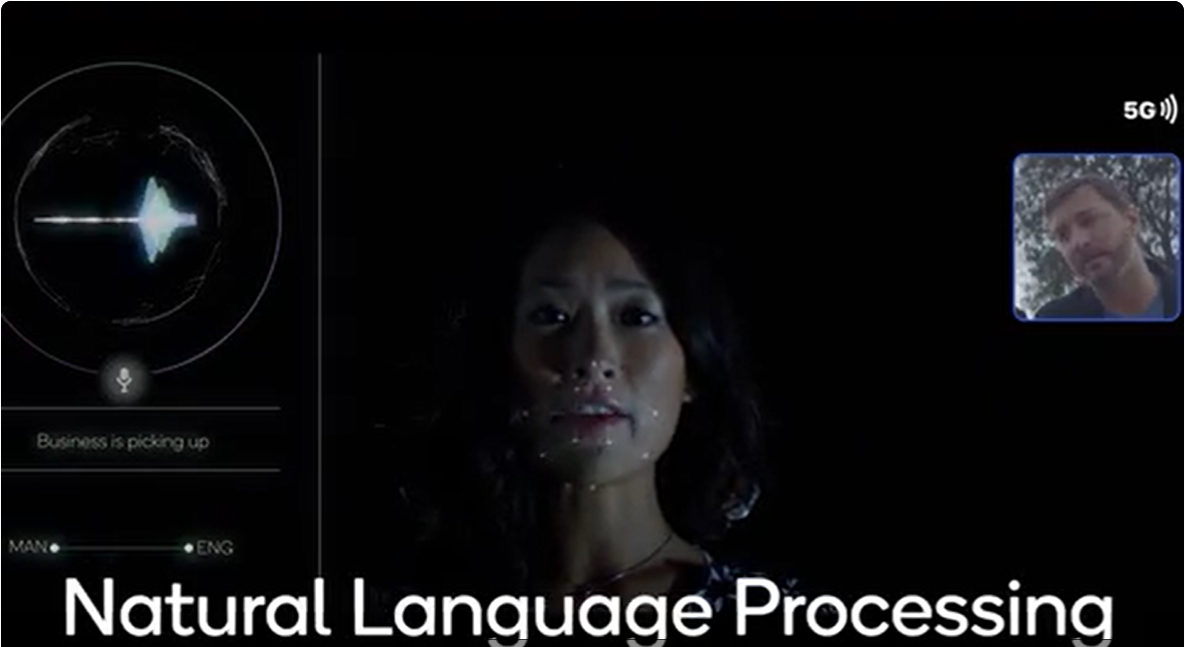
\includegraphics[width=1\columnwidth]{4.png}
            \end{figure}
            \begin{figure}[H]
                \centering
                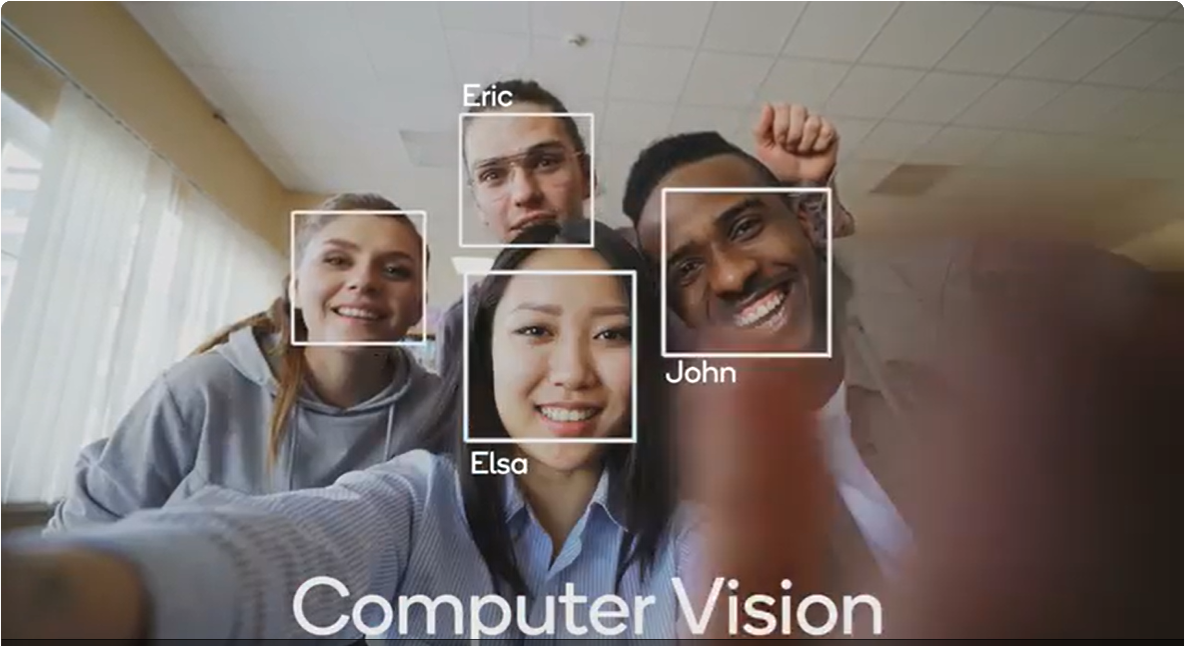
\includegraphics[width=1\columnwidth]{5.png}
            \end{figure}
        \end{column}
        \begin{column}{0.5\linewidth}
            Application support: Cloud AI
            \begin{itemize}
                \scriptsize
                \item Industry-leading 5G connectivity by Qualcomm Snapdragon X55 Modem-RF System
                \item Application and video processing on Qualcomm Snapdragon 865 Modular Platform
                \item Development kit supports leading software stacks including Pytorch, Glow, Tensorflow, Keras, and ONNX \cite{qualcomm}
            \end{itemize}
            Application targets:
            \begin{itemize}
                \item Natural Language Processing
                \item eXtended Reality
                \item Translations
                \item Computer Vision
            \end{itemize}
        \end{column}
    \end{columns}
\end{frame}
\section{Product Architecture}
\begin{frame}{Product Architecture}
    \begin{center}
        High performance, low latency, low power, datacenter to edge
    \end{center}
    \begin{figure}[H]
        \centering
        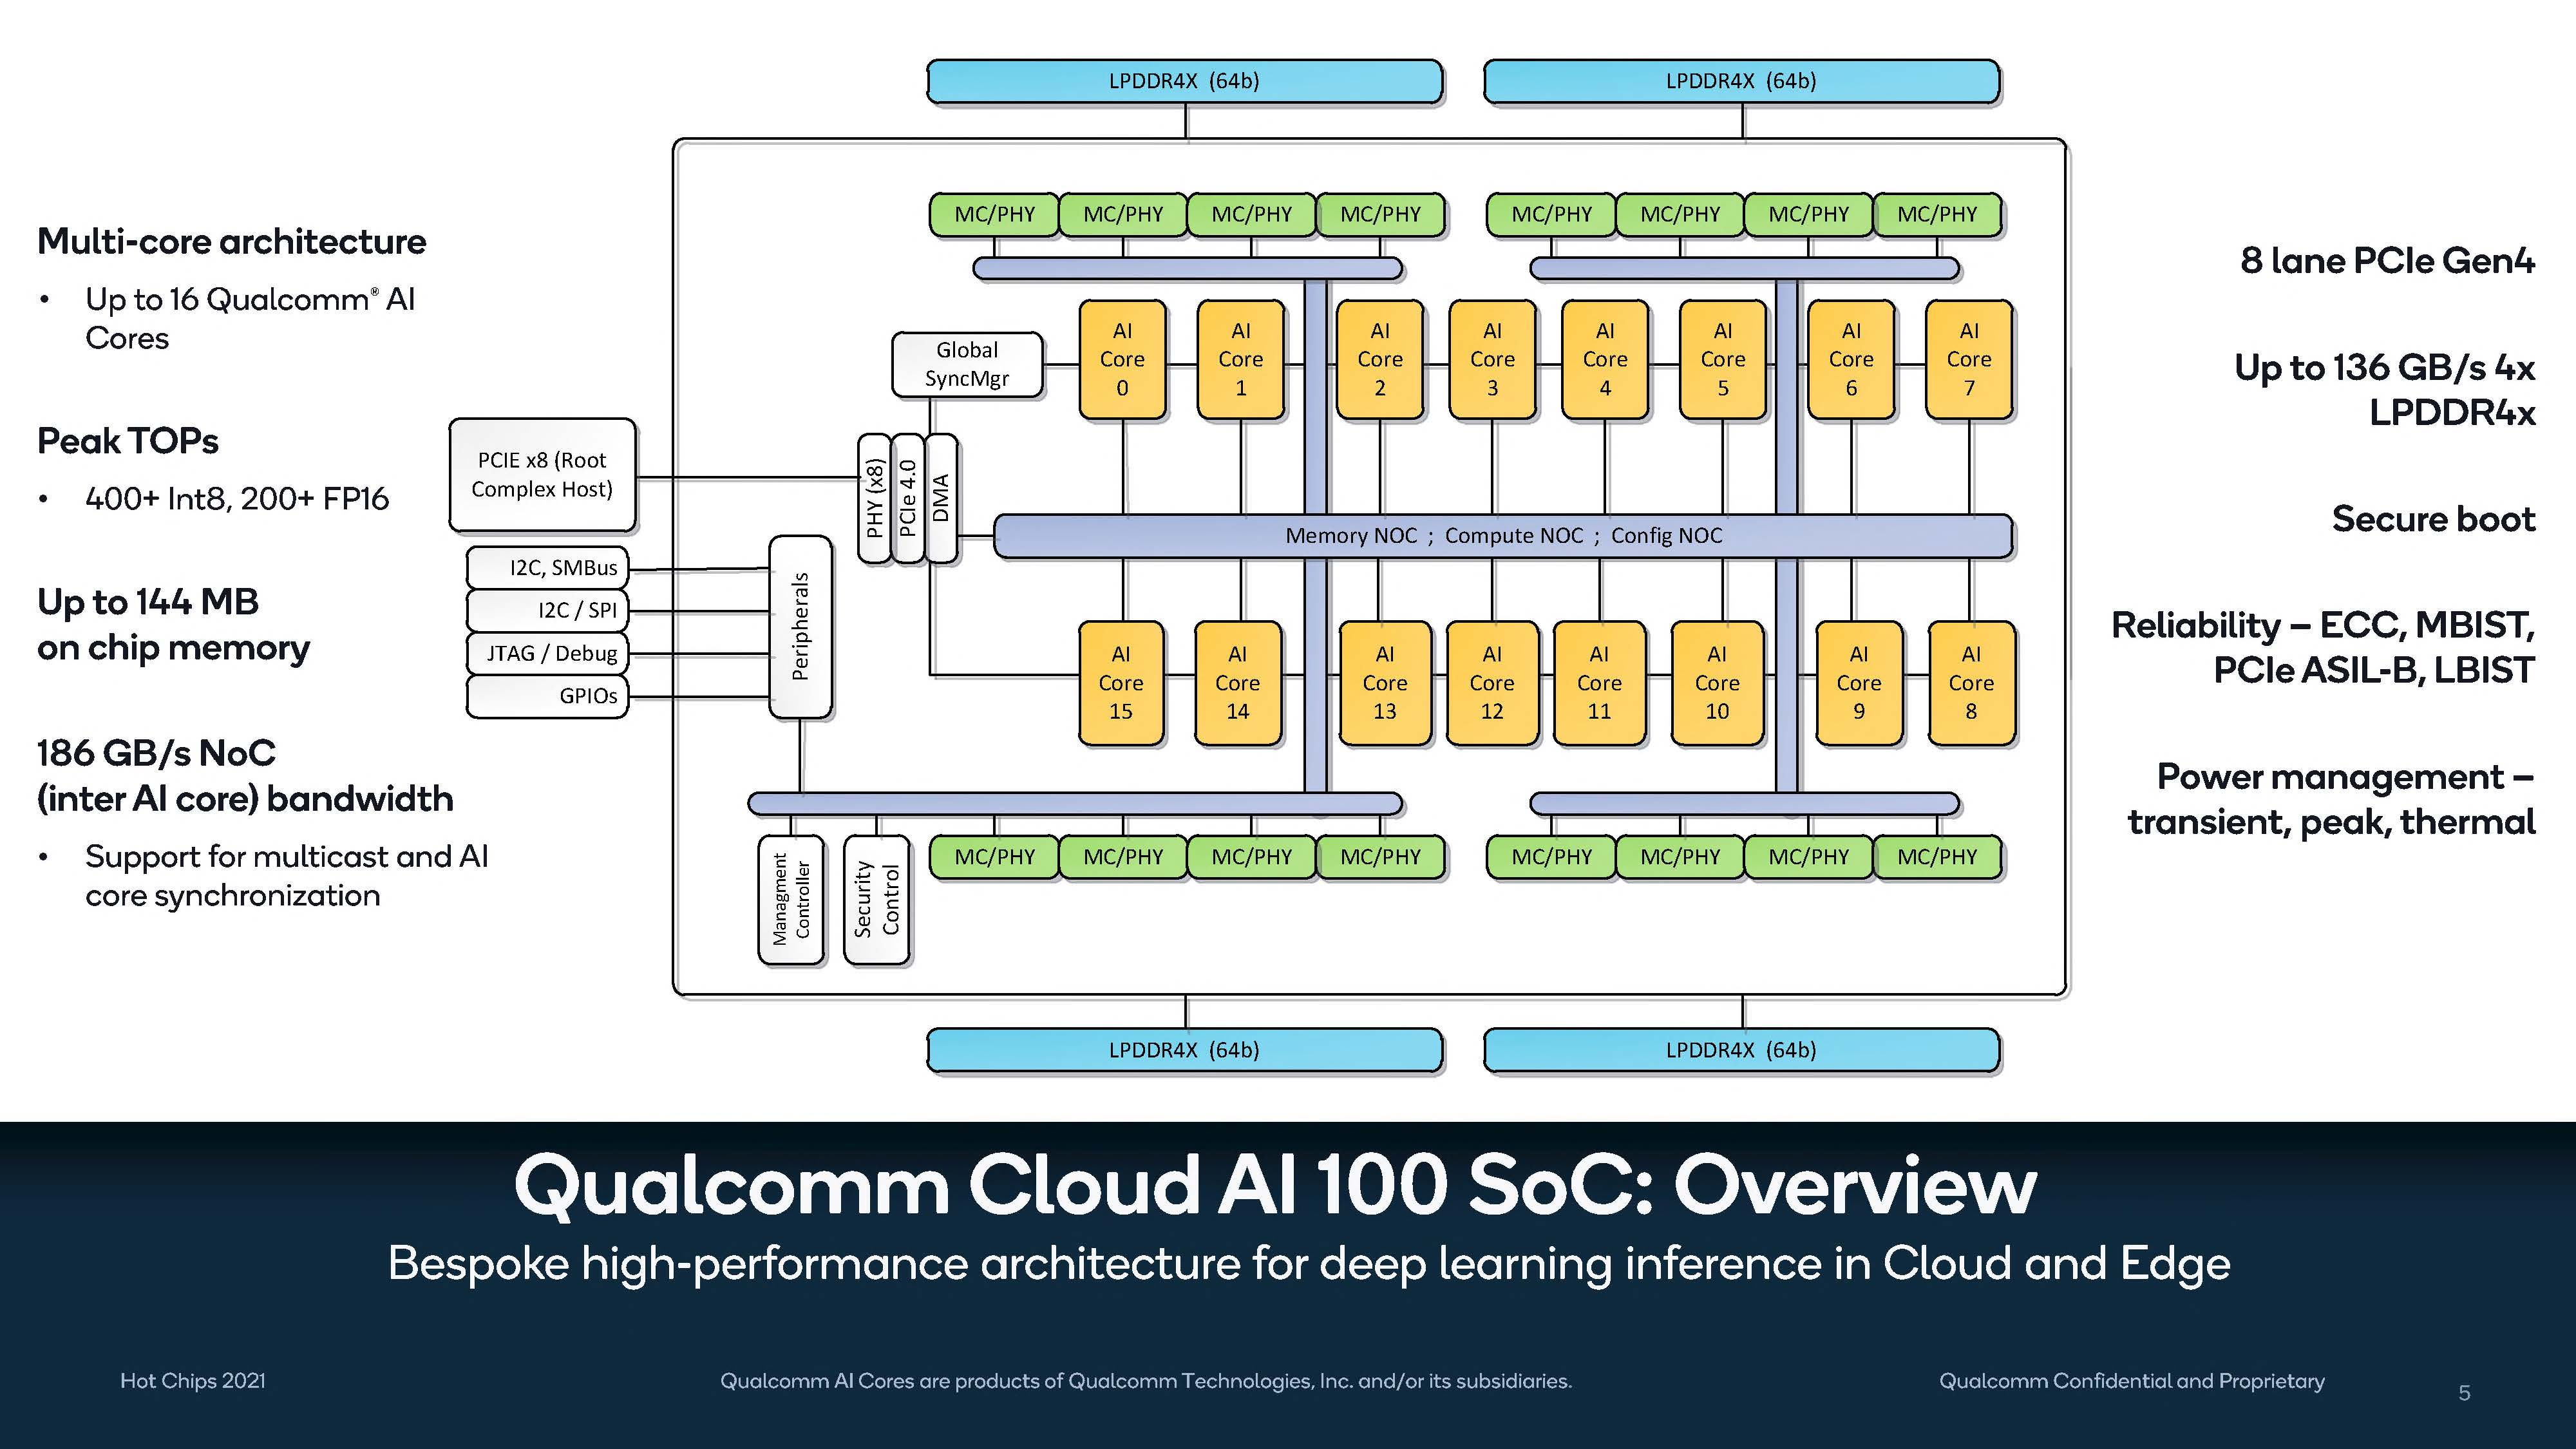
\includegraphics[width=1\textwidth]{1.jpg}
    \end{figure}
\end{frame}
\section{Main Features}
\begin{frame}{Main Features}{Qualcomm AI Core}
    \begin{columns}
        \begin{column}{0.4\linewidth}
            \begin{figure}[H]
                \centering
                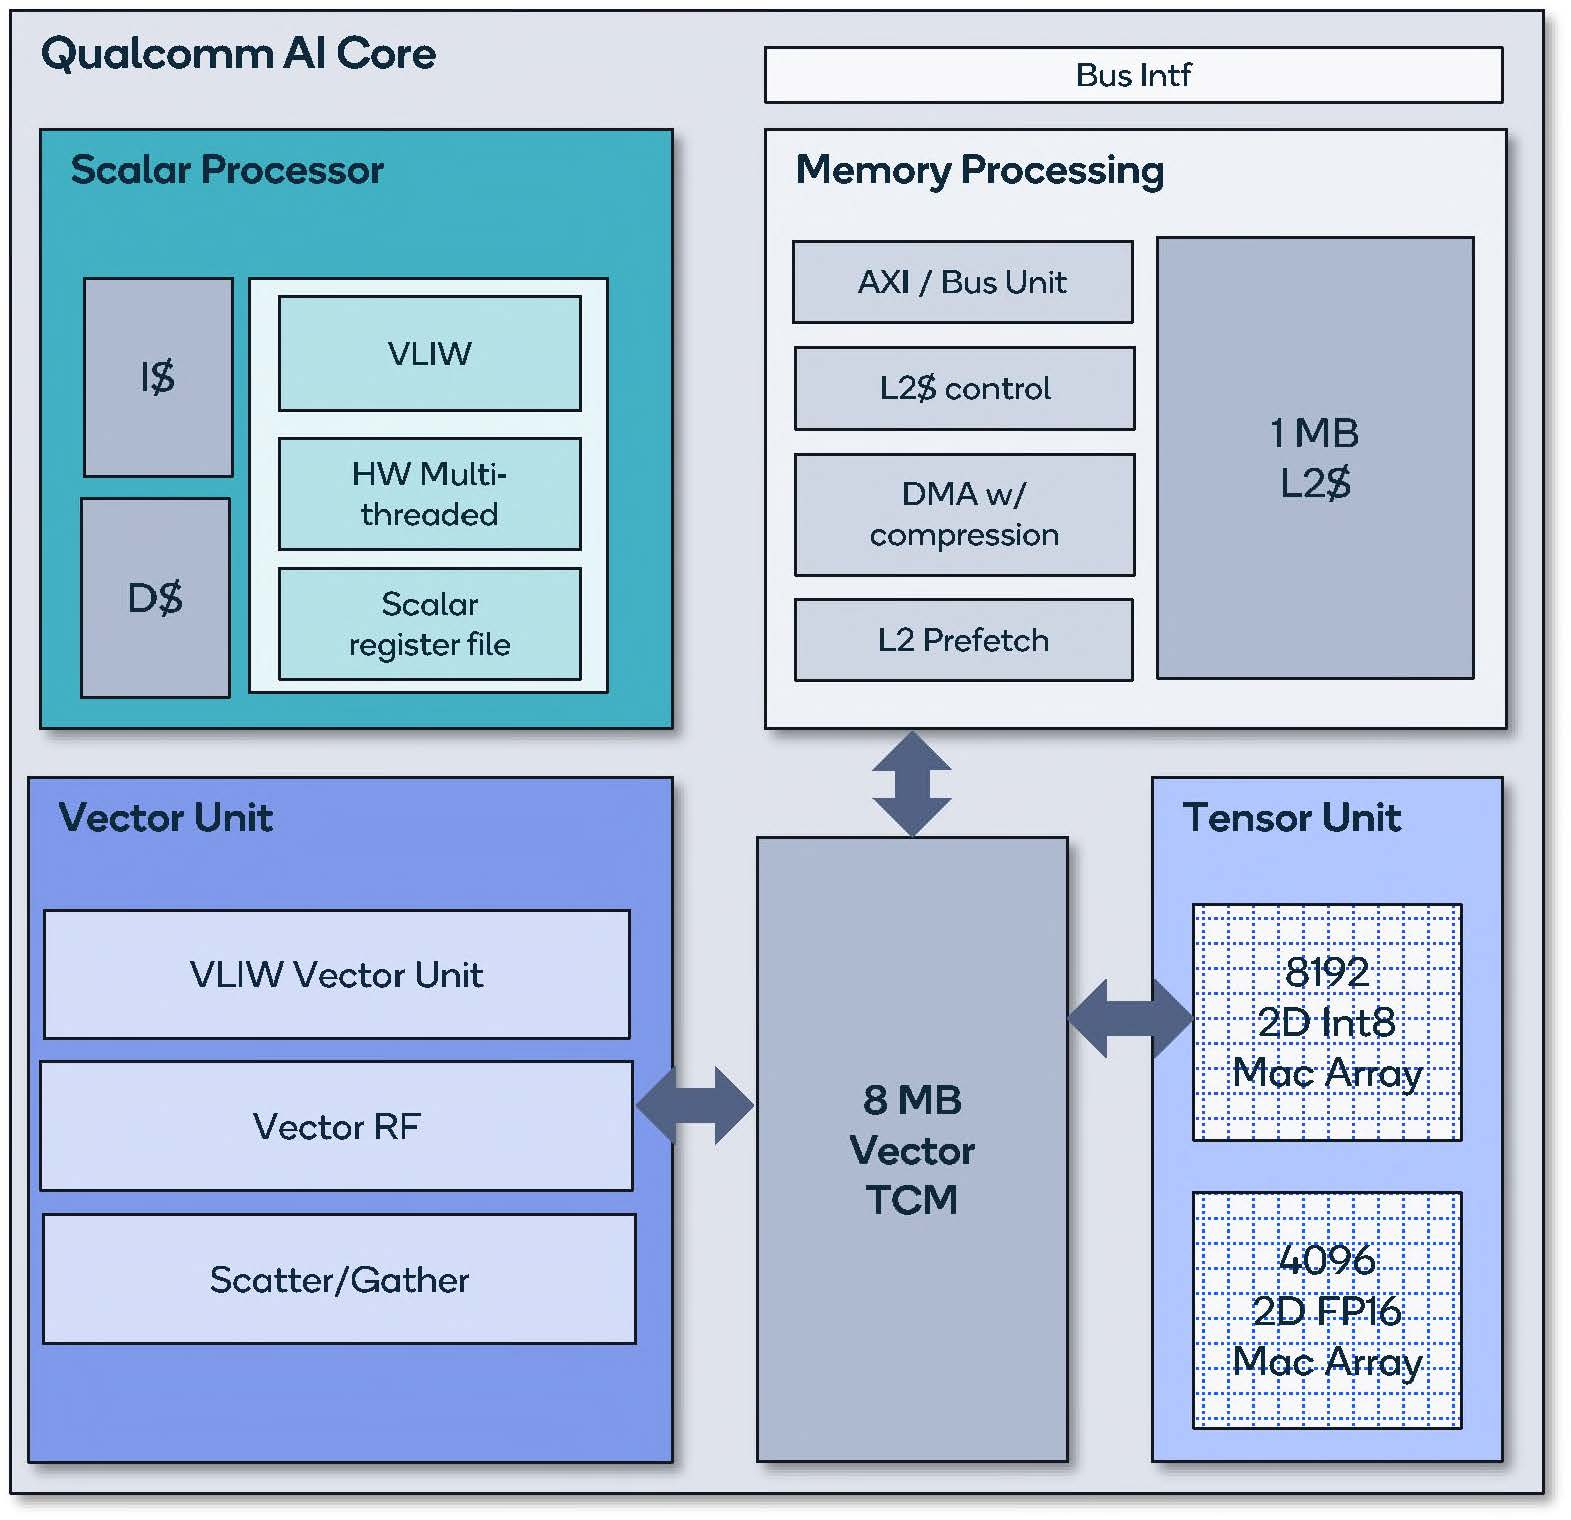
\includegraphics[width=0.8\columnwidth]{8.jpg}
            \end{figure}
        \end{column}
        \begin{column}{0.6\linewidth}
            \begin{itemize}
                \small
                \item Scalar - VLIW architecture
                \item Vector tightly couple memory (VTCM)
                \item Vector unit
                \item Tensor unit
            \end{itemize}
            \begin{table}[H]
                \centering
                \scriptsize
                \begin{tabular}{|c|c|c|c|}
                    \hline
                    SoC Power&12.05 W&19.74 W&69.26W\\
                    \hline
                    TOPs&149.01&196.64&363.02\\
                    \hline
                    SoC TOPs/W&12.37&9.98&5.24\\
                    \hline
                \end{tabular}
                \caption{Performance and power measured \cite{chatha2021qualcomm}.}
            \end{table}
        \end{column}
    \end{columns}
\end{frame}
\section{Specifications}
\begin{frame}{Specifications}
    \begin{columns}
        \begin{column}{0.4\linewidth}
            \begin{figure}[H]
                \centering
                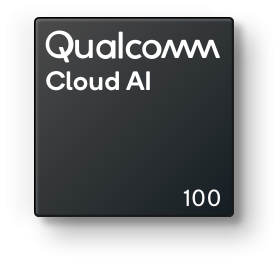
\includegraphics[width=0.8\columnwidth]{6.png}
            \end{figure}
        \end{column}
        \begin{column}{0.6\linewidth}
            \begin{itemize}
                \small
                \item Data Types: FP16, INT8, INT16, FP32
                \item On Die SRAM: 144MB (9MB Each AI Core)
                \item AI Cores: Up to 16
                \item Process Node and Technology: 7 nm
                \item Card: Dual M.2 (edge): 70 TOPS\@15W TDP, Dual M.2: 200 TOPS\@ 25W TDP, PCIe: 400 TOPS\@ 75W TDP\\
                On Card DRAM: Up to 32GB w/ 4x64 LPDDR4x \@ 2.1GHz \cite{qualcomm100}
            \end{itemize}
        \end{column}
    \end{columns}
\end{frame}
\section{Major Uniqueness}
\begin{frame}{Major Uniqueness}{Parallelization trade-offs}
    \begin{figure}[H]
        \centering
        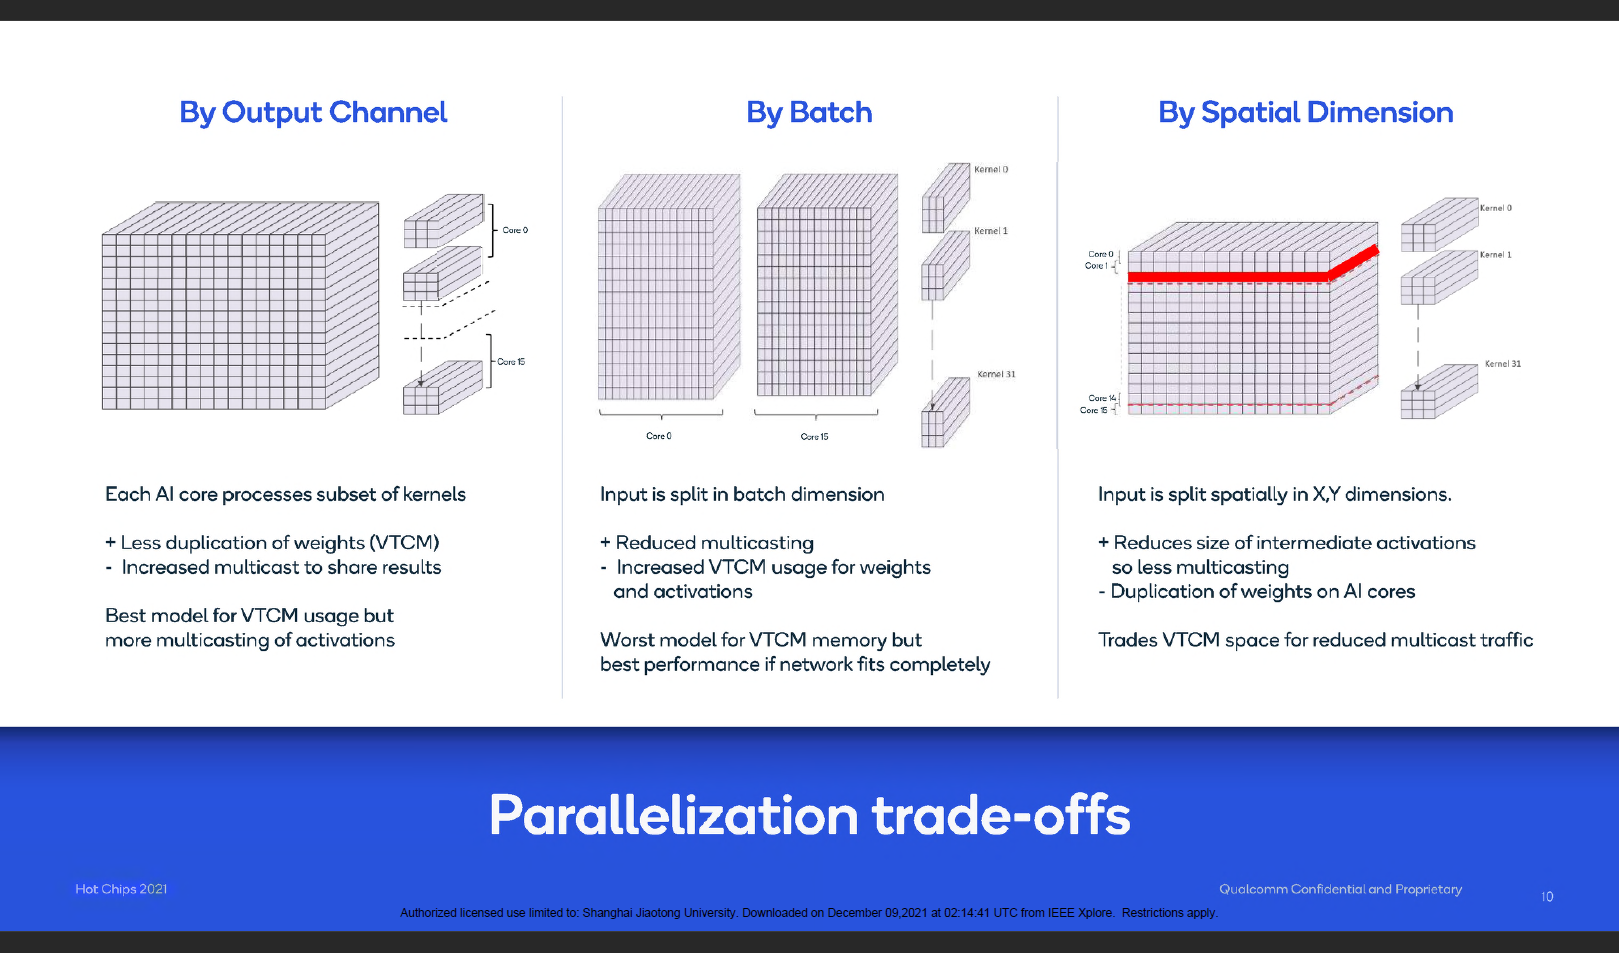
\includegraphics[width=1\textwidth]{7.png}
    \end{figure}
\end{frame}
\section{Reference}
\begin{frame}{Reference}
    \printbibliography
\end{frame}
\section{Thanks}
\begin{frame}
\begin{center}
    \Huge Thanks!
\end{center}
\end{frame}
\end{document}
